\documentclass[12pt, a4paper, twocolumn]{article}

\usepackage{color}
\pagecolor{white}
\usepackage{xspace}
%\usepackage{numprint}
%\usepackage{url}
%\usepackage{times}
%\usepackage{caption}
\usepackage{titling}
%\usepackage{titlesec}
\usepackage{sectsty}
%\sectionfont{\centering}
\usepackage{url}
\usepackage{float}
%\usepakcage{graphicx}
\usepackage{array}
\usepackage[hang,scriptsize,tight,nooneline]{subfigure}

%\usepackage{helvet}
%\renewcommand{\familydefault}{\sfdefault}

%\renewcommand{\familydefault}{\sfdefault}
%\normalfont

\usepackage{tgtermes}
\usepackage{enumitem}

\usepackage{xspace}
\usepackage[pdftex]{graphicx}

\newcolumntype{L}[1]{>{\raggedright\let\newline\\\arraybackslash\hspace{0pt}}m{#1}}
\newcolumntype{C}[1]{>{\centering\let\newline\\\arraybackslash\hspace{0pt}}m{#1}}
\newcolumntype{R}[1]{>{\raggedleft\let\newline\\\arraybackslash\hspace{0pt}}m{#1}}

%\titleformat{\section}
%  {\normalfont\Large\bfseries\centering}{\thesection}{1em}{}
    
\setlength{\droptitle}{-10em}
%\usepackage[a4paper]{geometry}
\usepackage[top=1.5in, bottom=1.5in, left=1in, right=1in]{geometry}
%\usepackage[utf8]{inputenc}
%\newcommand{\fixme}[1]{{\bf\textcolor{red}{[#1]}}}


\begin{document}
\title{\bf{BP STEP-UP \\ Backpressure-based routing protocol}}
\author{Sangeetha Abdu Jyothi, Gourav Khaneja}
\date{}
\maketitle

\label{sec:abstract}
\begin{center}
\section*{Abstract}
\end{center}

Shortest path routing schemes can lead to hot-spots or bottlenecks on some links, even when resources remain under-utilized elsewhere in the network. Hence, adapting the routing to network conditions through Traffic Engineering (TE) is essential for the efficient use of network resources. For this purpose, Internet Service Providers (ISPs) currently deploy TE over routing protocols, using techniques such as Multi-Protocol Label Switching (MPLS). However, such a deployment generate additional protocol overhead and have high reaction time to changes in the network traffic. Integrating TE capabilities with the routing scheme can bring about faster reaction to traffic variations as well as better utilization of resources. Our project involves developing and testing a distributed routing protocol capable of handling traffic variations in the network. The proposed protocol, based on the idea of backpressure routing, will route traffic along the best path based on conventional routing metrics (path length) as well as the congestion in the network.

\label{sec:intro}


%\begin{center}
\section{Introduction}
%\end{center}

Distributed systems face a wide array of challenges such as maintaining consistency, availability, resiliency to failure etc.  While an ideal distributed system should tackle all of these challenges effectively, this is not feasible in practice. Each system is forced to make trade-offs on various aspects of the design. However, as distributed systems are designed to serve specific environments, we can optimize the system to tackle only those issues that are critical to the intended environment. Networks constitute one of the most popular and widely used distributed systems, and the networking domain presents us with a unique array of challenges. Our project attempts to solve the problem of traffic engineering in networks by extending existing ideas.

Routing decisions of shortest path routing protocols are solely based on pre-assigned costs in the network and are agnostic to the real traffic. This can lead to congestion in some parts of the network and under-utilization elsewhere. We can achieve greater responsiveness to traffic variations and freedom from hot-spots by relying on protocols that combine distance information with knowledge about congestion in the network. 

Backpressure routing protocol~\cite{BP-orig} is based on the idea that queue lengths provide direct indication of congestion in the network. Each node in the network decides the next hop for incoming traffic by comparing its queue length with that of its neighbors. The largest difference in queue length, i.e. the largest gradient, will occur along the best path towards destination. Thus, each node forwards traffic based on queue length information received from its immediate neighbors. 

Backpressure routing scheme is throughput optimal -- if the incoming traffic is within the capacity region of the network, the protocol will route it successfully. In spite of its throughput efficiency, backpressure protocol is not widely used in practice due to several limitations. First, the protocol does not consider path lengths. Forwarding decisions are solely based on local congestion information. This causes routing loops and delays in the network. Second, each node has to maintain separate queues for every destination in the network. This is impractical for conventional switches with limited buffer space. However, the protocol does provide interesting features such as throughput-optimal routing and congestion-awareness. 

%In particular, one of the variants~\cite{Srikant3} also obviates the need for multiple queues per node.

Recently, several ideas have been proposed ~\cite{Srikant3, Austin1} that combine the notion of shortest path routing with backpressure protocol. This opens an exciting arena for congestion-aware shortest path routing. However, the efficiency of these algorithms has not been tested extensively by the limited simulations performed on it. The algorithmic foundation also requires further work to be expanded into a fully-functional distributed protocol, suitable for practical realization. 

We devised and implemented BP STEP-UP, a backpressure-based distributed routing protocol, which involves six optimizations that improves the performance of the basic protocol significantly. 
These optimizations are:

\begin{itemize}[noitemsep]
\item[] \textbf{\large S} hadow queues ~\cite{Srikant3}
\item[] \textbf{\large T} hreshold for back-pressure ~\cite{Srikant3}
\item[] \textbf{\large E} xpansion of shadow traffic ~\cite{Srikant3}
\item[] \textbf{\large P} roportional splitting \\
\item[] \textbf{\large U} ni-hop optimization
\item[] \textbf{\large P} ath length based initialization
\end{itemize}
 
We developed a Java-based distributed implementation of BP STEP-UP and tested the protocol on OCEAN testbed at UIUC. We studied the impact of each optimization and showed that BP STEP-UP can reduce link congestion by upto 50\% and improve the convergence time by upto 30\%.
%\bigskip
\label{sec:related}
\section{Related work}

Tassiulas and Ephremides discovered that queue length is an indicator of congestion in the network while exploring max-weight scheduling in wireless networks and leveraged this information for maximizing throughput in wireless environment~\cite{BP-orig}. The original backpressure algorithm was the extension of max-weight scheduling algorithm in multi-hop wireless networks. This algorithm was independently discovered as a solution to multi-commodity flow problem by Leighton et. al.~\cite{Leighton1}. McKeown et al.~\cite{nick1} extended this idea to input-queued switches and introduced the notion of throughput optimal routing in wired networks. Although the idea of backpressure routing had been introduced more than two decades ago, it is not widely used in practice due to poor delay performance caused by routing loops. In spite of its shortcomings, we propose to explore this direction further since backpressure is the only proven technique that can achieve throughput optimal routing in a distributed manner without a priori knowledge about the traffic patterns. While protocols such as modified OSPF~\cite{mOSPF}, DEFT~\cite{DEFT}, PEFT ~\cite{PEFT} etc. combine traffic engineering with routing, they involve centralized computation which prevents a completely distributed deployment. On the other hand, backpressure algorithm can be implemented as a totally decentralized protocol.

Several modifications have been introduced to improve the performance of the traditional backpressure algorithm. Backpressure Control Protocol~\cite{BCP} used in sensor networks replaces FIFO service with LIFO service to improve delay performance. The importance of using shortest paths with backpressure to reduce delay was first put forward by Neely et al.~\cite{Neely1}. Another work~\cite{SP1} also notes that lack of a metric that indicates closeness to the destination, is a cause for poor delay performance of opportunistic protocols such as backpressure. Multiple variations of backpressure protocol that rely on the notion of shortest paths to reduce delays have been proposed after Neely~\cite{Neely1} introduced the idea. Ying et al.~\cite{Austin1} uses the shortest path information by maintaining additional queues at each node corresponding to hop-counts. Packet-by-packet adaptive routing ~\cite{Srikant3} also combines shortest path and backpressure routing to achieve high performance. It provides an elegant solution for separating routing and scheduling by introducing the notion of shadow packets. Separating the backpressure computation from the real packet routing using shadow packets was first proposed in ~\cite{Srikant1} and ~\cite{Srikant2}. The notion of backpressure has also been explicitly combined with shortest path routing in ~\cite{BP-lcn}.

As an optimization, we intend to use the idea of proportional sharing of links introduced by Walton~\cite{walton} to speed up the convergence of backpressure routing.
\label{sec:backPressure}
\section{Backpressure routing}
The goal of our project is to develop a distributed throughput optimal routing scheme. A throughput-optimal routing scheme implies that if the demand on the network, i.e, the set of flow requirements, is less than the available capacity in the network, the routing and scheduling scheme should be capable of handling the traffic with minimal delay. In order to achieve our primary goal, we rely on the technique of backpressure routing. In this section, we describe the network model used for the analysis of backpressure routing. Next, we introduce the original backpressure protocol, existing variations of it and our modifications.

\subsection{Network model}
The network model consists of a directed graph $G=(N,E)$ where $N$ is the set of nodes and $E$ is the set of directed edges. A bi-directional link in the network is represented by two directed edges in the graph. A directed edge that can send packets from node $n$ to node $j$ is denoted by $(nj) \epsilon E$. We assume that the time is slotted for the initial derivation. Capacity of the link $(nj)$ is represented by $c_{nj}$, which is the maximum number of packets that can be transmitted in one time-slot.

The set of flows in the network is denoted by $F$. Although each flow has a specific source and destination in the network, no paths are specified. Each flow has a specific input rate denoted by $x_{f}$. $\mu_{nj}^{d}$ is used to represent the rate allocated to flows destined to node $d$ on link $(nj)$.

\subsection{Original Backpressure Protocol}
In this section, we describe the basic backpressure algorithm proposed in \cite{BP-orig} and its shortcomings. The original backpressure protocol put forward an iterative algorithm that combines routing and scheduling. Each node in the network maintains a separate queue for every destination in the network. The backpressure on a link for a particular destination in a given time slot is 
\begin{equation}
w_{nj}^{d}[t] = Q_{nd}[t] - Q_{jd}[t]
\end{equation}
where $Q_{nd}[t]$ denotes the queue length for destination $d$ on node $n$ at time-slot $t$. In each time slot, a single destination is chosen for transmission based on the largest backpressure. If multiple destinations have the same backpressure, one of them is chosen randomly. The chosen destination is given by

\begin{equation}
d^{*}_{nj}[t] = arg\:max\;{w_{nj}^{d}[t]}
\end{equation}

At time $t$, for each link $(nj)$, $c_{nj}$ packets are transmitted from $Q_{nd^{*}}$ and added to $Q_{jd^{*}}$. Throughput optimality of this scheme is proved in \cite{BP-orig}. But this protocol has several disadvantages. It requires per-destination queues at all nodes in the network. The protocol forces a flow to explore all paths in the network before converging on the best paths. This can lead to routing loops, large queues and hence, large delays in the network. Due to these constraints, backpressure routing is not used in practice.

%
%\subsection{Previous modifications}
%Several modifications have been proposed to improve the performance of backpressure routing protocol. We focus on Packet-by-packet Adaptive Routing for Networks (PARN)~\cite{Srikant3}, In order to improve the performance of the original backpressure routing protocol, PARN introduces the following modifications.
%
% PARN requires only per-neighbor queues at each node. Instead of per-destination queues, PARN maintains counters called shadow queues. When a flow adds packets at the rate $x_{f}$ to the real queue, shadow queue counters are incremented at a rate $ x_{f} * (1+\epsilon)$. This additional pressure on shadow queues force faster convergence in the shadow queue domain. While the basic backpressure allow packet transmission when the backpressure is positive, PARN requires that the backpressure be greater than a threshold of M. This forces the flows to follow shorter paths.
%
%We derive inspiration from these modifications - separation of real packets and backpressure computation, stressing the shadow queues for faster convergence and forcing the packets through a shorter path. We borrow these ideas in the design of BP STEP-UP.

\subsection{BP STEP-UP}
The original backpressure protocol was introduced more than two decades ago. Although it has several desirable properties, practical deployment of the protocol has remained infeasible over the years. After analyzing the performance of basic backpressure protocol and PARN~\cite{Srikant3}, we design BP STEP-UP which includes six optimizations over the basic protocol that enable us to develop it into a distributed system. These optimizations are:
\begin{itemize}[noitemsep]
\item[] \textbf{\large S} hadow queues ~\cite{Srikant3}
\item[] \textbf{\large T} hreshold for back-pressure ~\cite{Srikant3}
\item[] \textbf{\large E} xpansion of shadow traffic ~\cite{Srikant3}
\item[] \textbf{\large P} roportional splitting \\
\item[] \textbf{\large U} ni-hop optimization
\item[] \textbf{\large P} ath length based initialization
\end{itemize}
Three of these optimizations are adapted from PARN~\cite{Srikant3} while the remaining three are new contributions. Next, we discuss each optimization in detail.


\begin{itemize}[leftmargin=*]
\item[] \textbf{Shadow queues} - Like PARN, BP STEP-UP maintains a single real queue per neighbor and separate counters per destination on each link called the shadow queues. This obviates the need for per-destination queues on router and allows practical deployment. In each iteration, real packets are transmitted from the real queue in FIFO order, while transmission from shadow queues follow backpressure algorithm. Packet transmission between shadow-queues manifest as a decrease in counter at the sender and an increase in counter at the receiver. Each link is also associated with a set of token buckets per destination~\cite{Srikant3}. A real packet is added to the real queue of that neighbor which has the smallest token bucket corresponding to the destination. A token bucket for a particular destination is incremented when a real packet with the same destination is added to the FIFO queue. It is decremented when shadow packets corresponding to that destination is sent. Thus, shadow queues perform the backpressure protocol and indirectly influences the scheduling of real packets through token buckets. The complexity of backpressure computations is shifted from real-packet transmissions to the shadow queues. A detailed description of the interaction between shadow queues and real queues can be found in ~\cite{Srikant3}.

\item[] \textbf{Threshold for Backpressure} - Shadow packets are transmitted for a single destination with the largest backpressure. However, even the largest backpressure might be a small value. This happens when a node and its neighbor has similar queue lengths for all destinations. In such cases, backpressure can oscillate between the nodes causing packets to travel to and fro on the link. In order to prevent this scenario, shadow packet transmissions are allowed only when the backpressure on the link exceeds a certain threshold.

\item[] \textbf{Expansion of shadow traffic} - When a flow adds packets at the rate $x_{f}$ to the real queue, shadow queue counters are incremented at a rate $ x_{f} * (1+\epsilon)$. This additional pressure on shadow queues force faster convergence in the shadow queue domain which, in turn, reduces looping of real packets. 

\item[] \textbf{Proportional splitting} - In the backpressure algorithm and its various modifications, a single destination is chosen for transmission at each time-slot. Intuitively, this does not provide us with a smooth transition in the queue lengths. The queue lengths of destinations fluctuate tremendously depending on $c_{nj}$. The chosen destination transmits $c_{nj}$ packets at each time-slot. As a result, it transitions from the highest backpressure destination to one with a very low backpressure and continues to oscillate between these two stages. To allow a smoother convergence through smoother transitions, we split the capacity proportionally across all destinations which have a positive backpressure. For example, if the link allows transmission of 100 shadow packets per time-slot, instead of sending all 100 packets corresponding to a single destination, the capacity of 100 can be proportionally shared across top $K$ destinations with the highest backpressure. Mathematically, we transition from a linear cost function to logarithmic cost function. This idea was initially proposed by Walton in a different context~\cite{walton}. We demonstrate that this approach significantly improves the performance of backpressure protocol and its variants.
   
\item[] \textbf{Uni-hop optimization} - This is a simple optimization in which packets are forwarded directly to the neighbor if it is the destination of the packet. The basic backpressure protocol relies on backpressure to forward a packet even when its destination is a neighbor. This optimization reduces the distance travelled by the packets in the network by directing packets towards their destination at the last hop.
 
   
\item[] \textbf{Path length based shadow queue initialization}  The initial value of shadow queue does not affect the correctness of the system. To take advantage of this, we initialize the shadow queue with a multiple of path length. Thus, we establish an initial backpressure that favors shortest path. This can reduce the convergence time significantly. We show that using explicit path length information is more useful than using an indirect metirc like the threshold M.

\end{itemize}
 

\label{impl}
\section{Implementation}

\begin{figure*}
\centering
\begin{minipage}[b]{0.45\linewidth}
	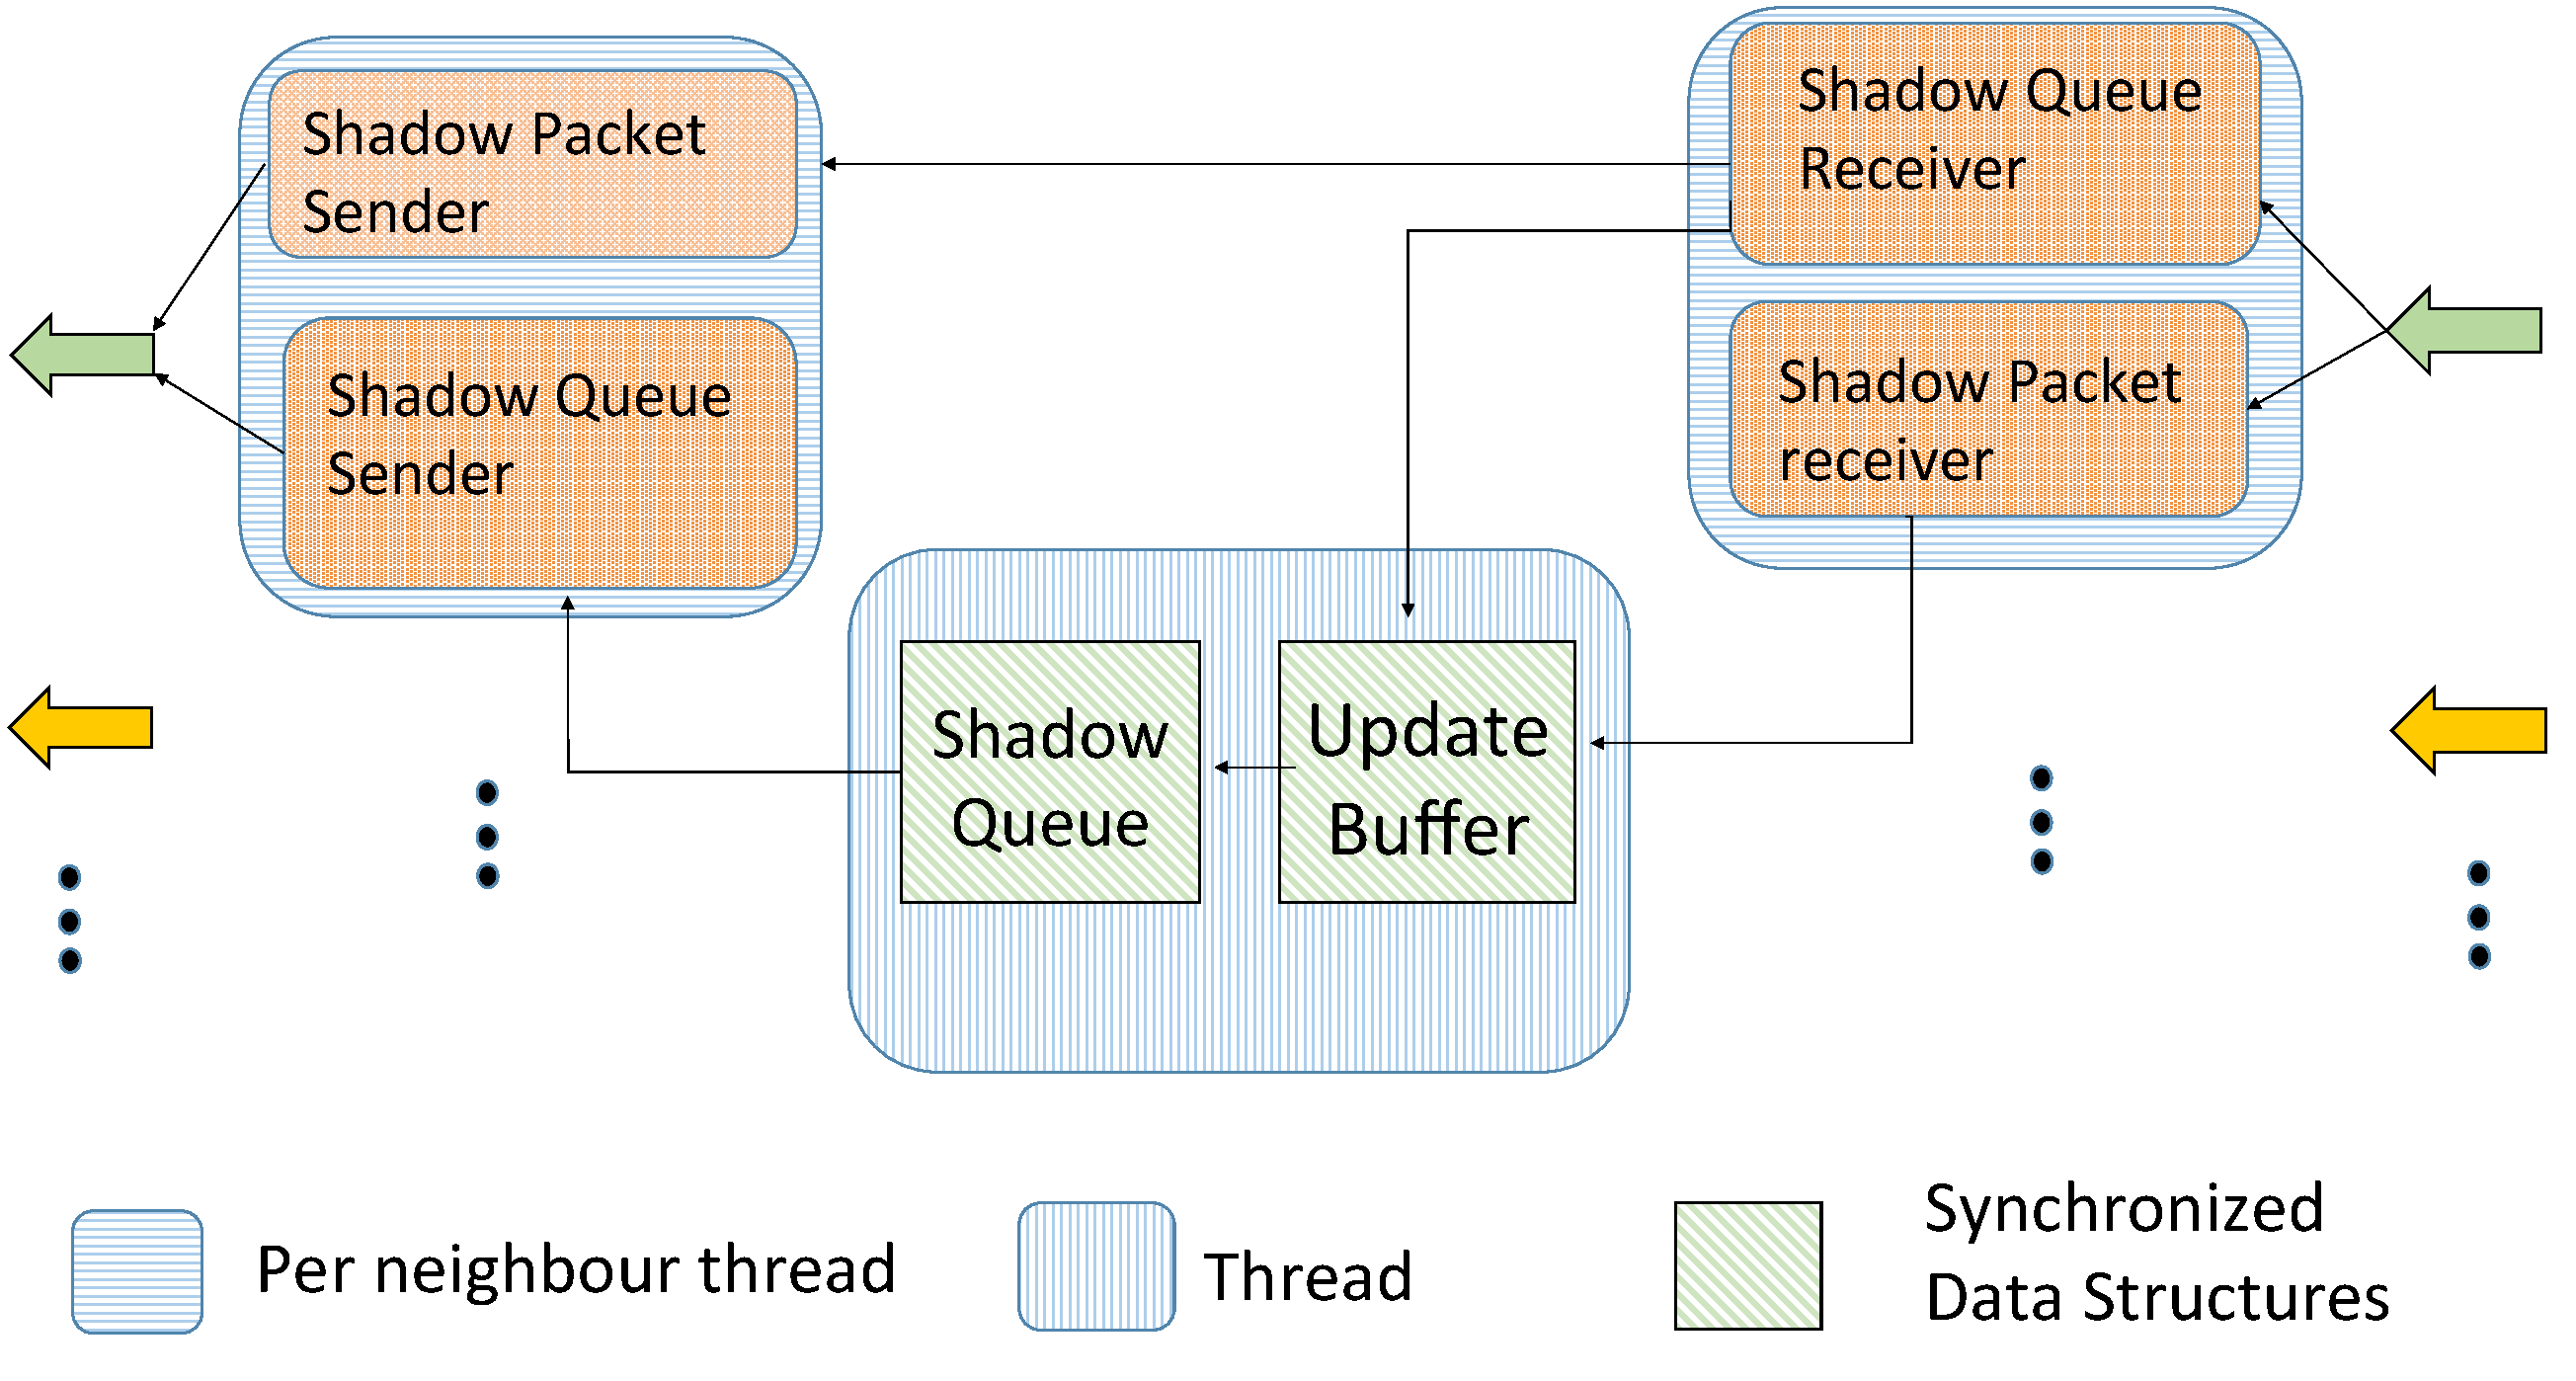
\includegraphics[width=2.4in]{./figures/controlpath2.pdf}
	\caption{Control path}
	\label{fig:control}
	\centering
	%\small Control path
\end{minipage}
\begin{minipage}[b]{0.45\linewidth}
	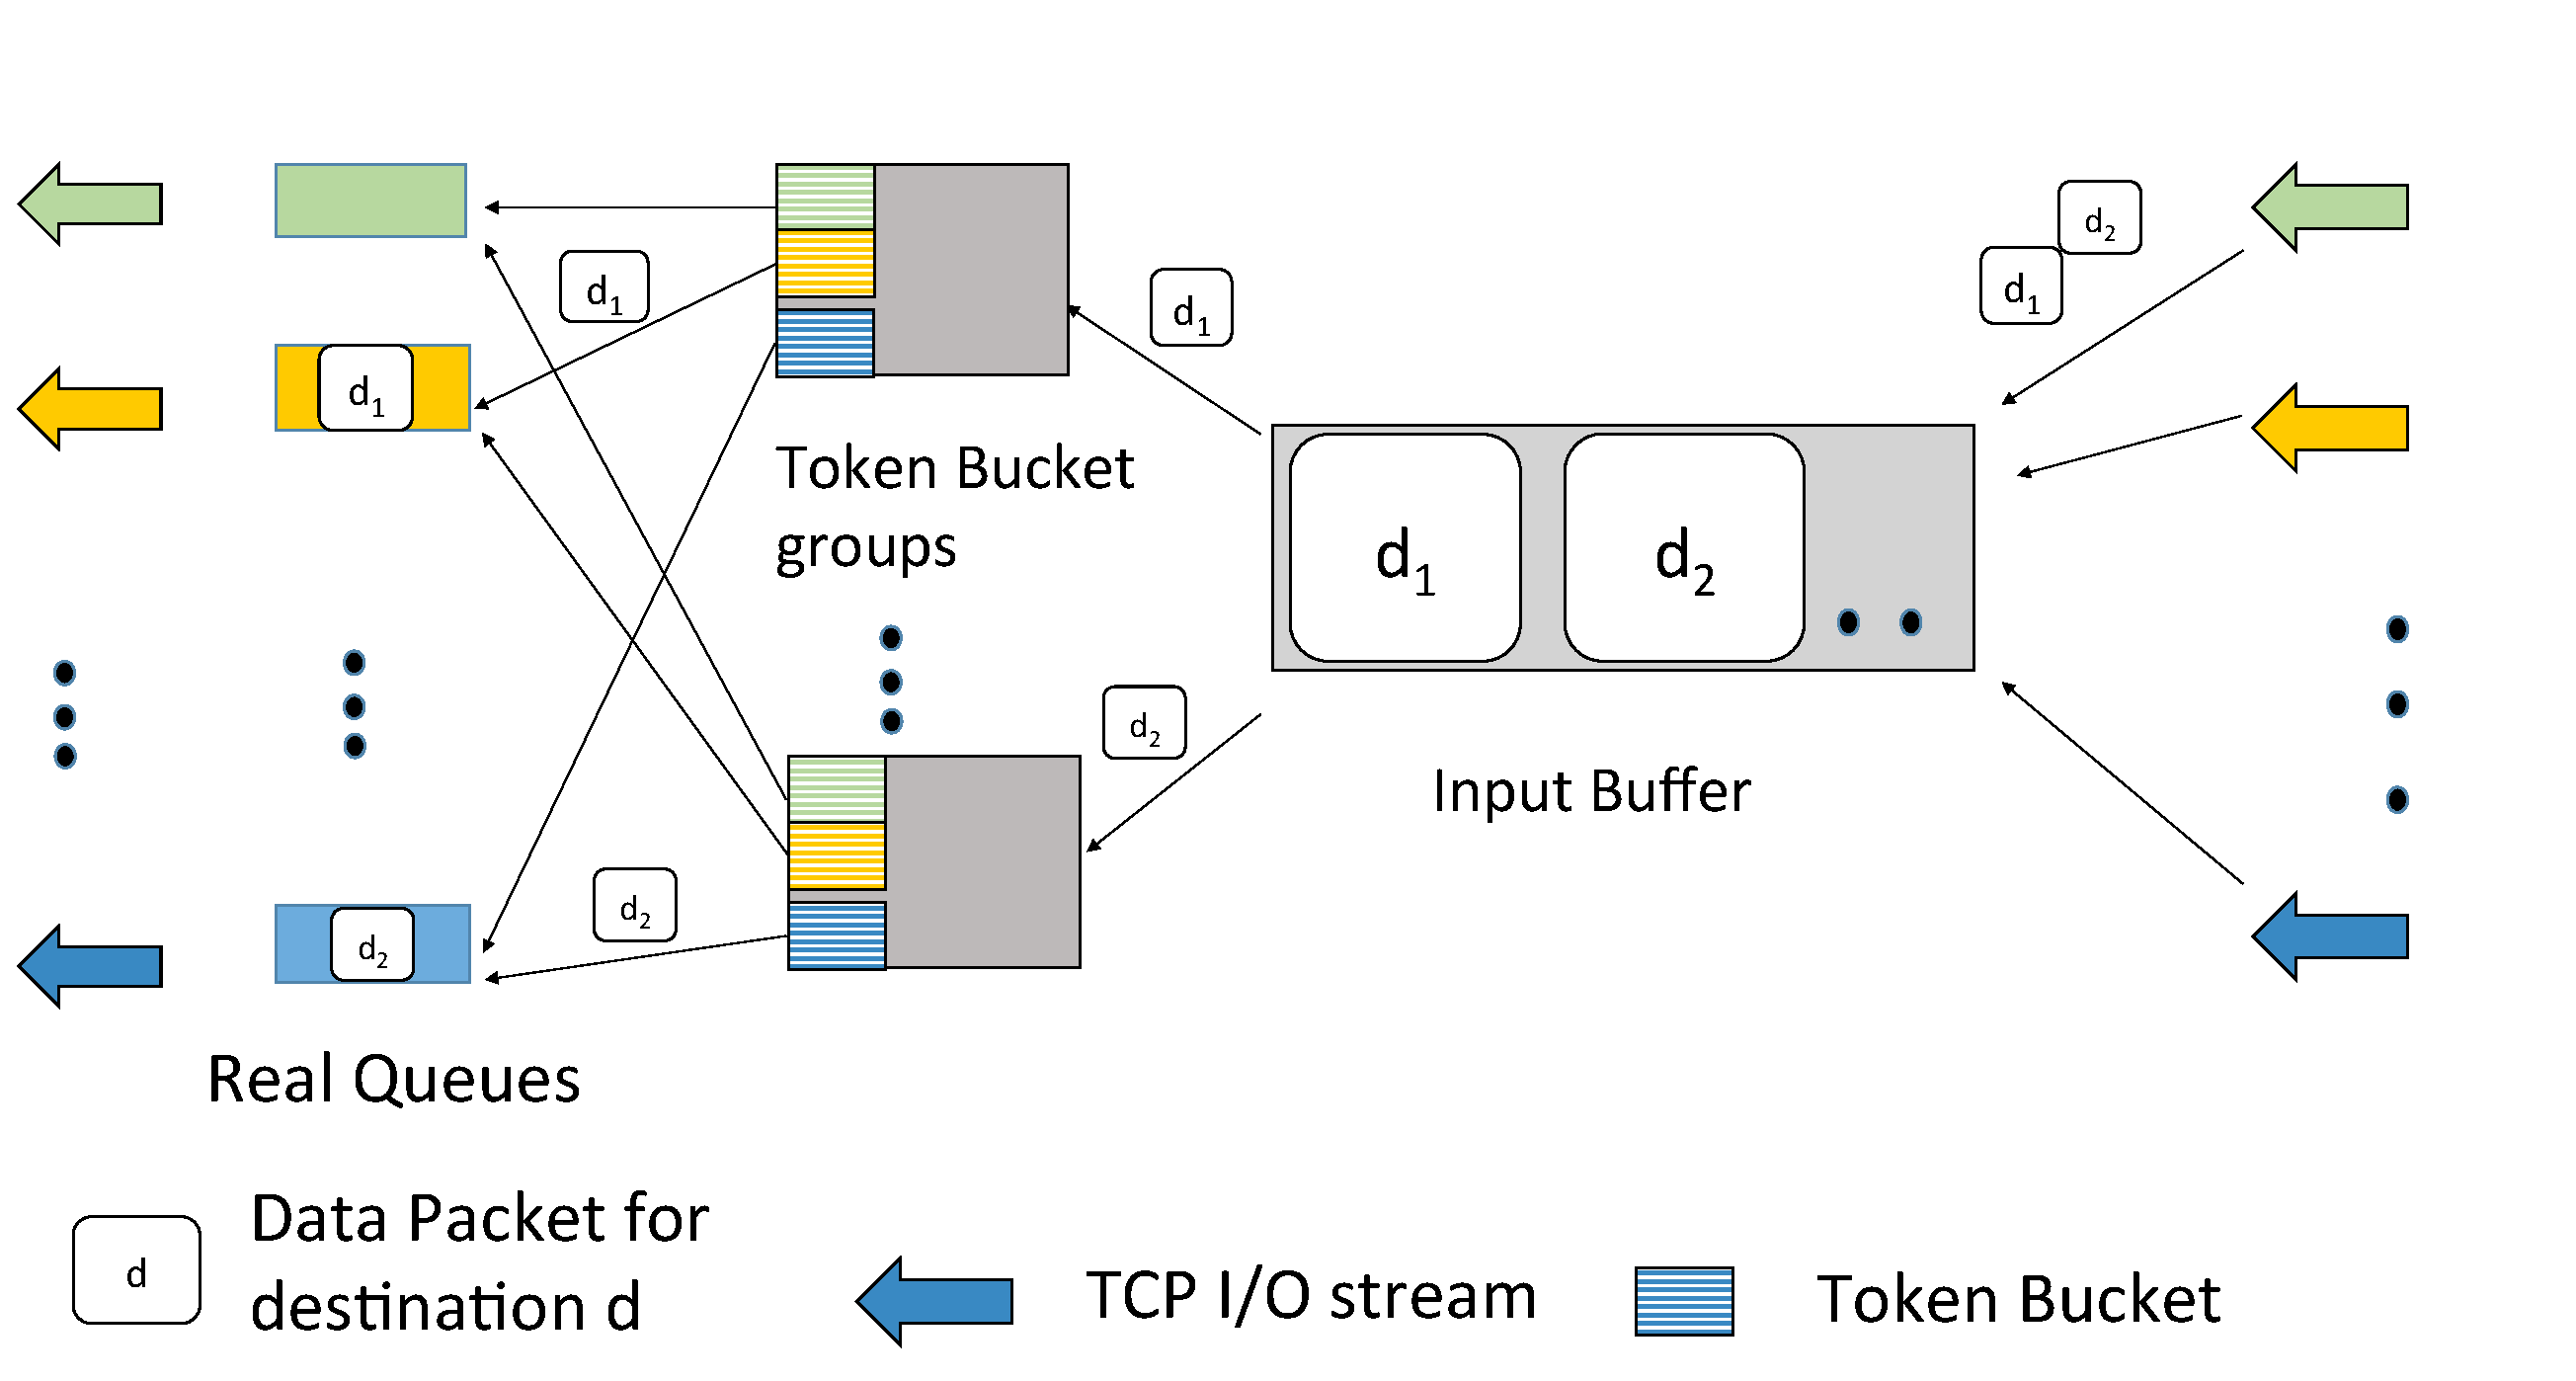
\includegraphics[width=2.4in]{./figures/datapath4.pdf}
	\caption{Data path}
	\label{fig:data} 
	\centering
	%\small Data path 
\end{minipage}
%\caption{\small Control path and data path in the real implementation}
%\label{fig:TCompare}
\end{figure*}


We implement the protocol as on overlay network over TCP/IP. We test the basic backpressure protocol as well as BP STEP-UP with different combinations of optimizations to identify the best one/combination. The rest of this section gives an overview of overlay node implementation. It consists of two parts - (a)Data Path which deals with routing and transmission of real packets from the FIFO queues and (b)Control Path which is responsible for transmission of shadow packets and exchange of information regarding shadow queues. 

\textbf{Data Path}(Figure~\ref{fig:data}) handles the routing and scheduling of Data packets. Each node maintains an incoming data channel per neighbor, each of which drains data packets into an \textit{input buffer} (FIFO queue) in a FIFO fashion. Packets from different channels may inter-mix in an arbitrary order depending on synchronization constructs of the \textit{input buffer}. Like incoming channels, outgoing data channels are maintained for each neighbor, each of which drains packets from corresponding \textit{real queue} in FIFO fashion. A system-wide thread transfers packets from \textit{input buffer} to an appropriate \textit{real queue} based on \textit{token buckets} ~\cite{Srikant3}. A \textit{token bucket group} is maintained for each destination, which contains \textit{token buckets} for each neighbor (or \textit{real queue}). A packet for destination \textit{d} goes to the smallest \textit{token bucket} in the corresponding group.

\textbf{Control Path} (Figure~\ref{fig:control}) describes the flow of control information i.e. number of shadow packets transferred and shadow queue length advertisements. Like data channels, incoming and outgoing control channels are maintained for each neighbor. Control information received from neighbors is buffered before it is applied to update nodes' own shadow queues. The way buffered updates are applied to shadow queues defines the synchronization construct. Waiting for updates from all the neighbors maps to slotted time assumption, which may result in high convergence time (since it is as slow as the slowest neighbor). The other extreme is to apply updates as soon as they are received, which is not proved to converge. We will test the system with different synchronization constructs. Note that updating shadow queue includes adjusting shadow queue lenghts, generating shadow packets (to be sent to neighbors) and updating token buckets, which determines the DataPath.

%\label{experiments}
\section{Experiments}

In this section, we present the performance comparison of various backpressure variants on our simulator and provide a brief overview of the real-world implementation. All experiments are carried out on a 12 core Intel Xeon CPU E5-1650 machine with 32GB RAM operating at 3.20GHz. We tested a variety of networks with two main traffic matrices - all-to-all traffic matrix and random permutation traffic matrix. All presented results are for n-dimensional hypercubes with all-to-all traffic matrix.

\subsection{Simulations}

\textbf{Basic backpressure algorithm}
\begin{figure}
%\centering
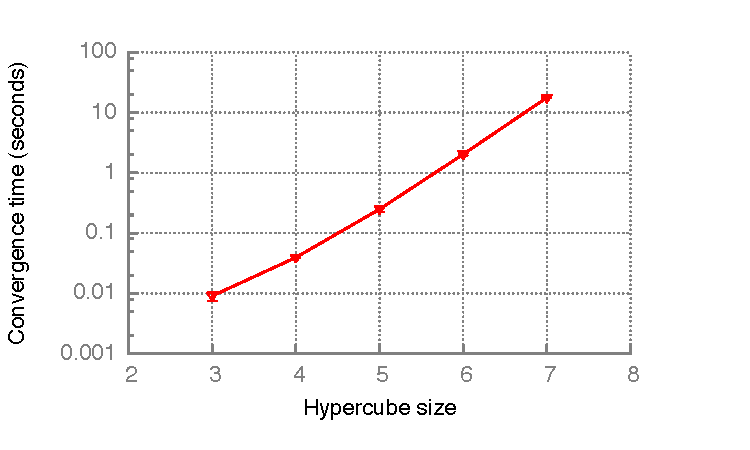
\includegraphics[width=3in, height=2in]{./figures/basic.pdf}
\caption{\small Performance of basic backpressure algorithm}
\label{fig:M_1}
\end{figure}

\textbf{Variation with epsilon}

\textbf{Variation with threshold}
In figure~\ref{fig:M_1},we observe that 
\begin{figure}
%\centering
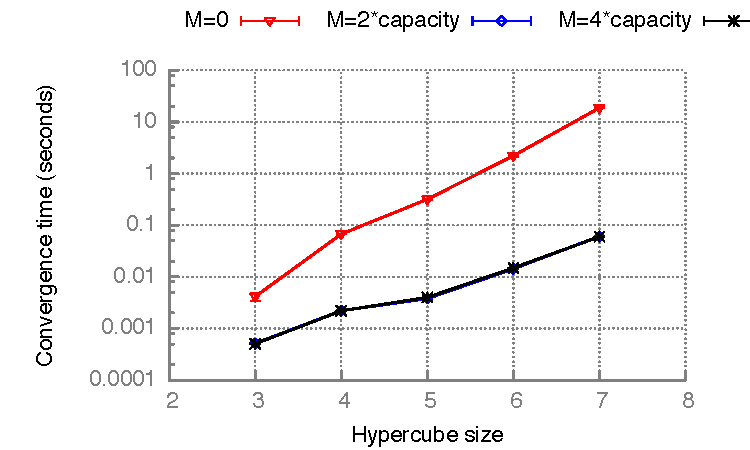
\includegraphics[width=3in, height=2in]{./figures/M_variation.pdf}
\caption{\small Variation of convergence time with M}
\label{fig:M_1}
\end{figure}


\subsection{Real implementation}




\section{Conclusion}
Implementation of throughput-optimal routing scheme presents a unique challenge in the domain of distributed systems. We need a system that can efficiently route traffic under varying loads with minimal delay and no apriori knowledge of the incoming flow rates. We propose to modify an exisiting idea and improve its performance to tackle this problem effectively.

We have built a simulator and tested existing and new variants of backpressure protocol. Combination of various optimization techniques allow us to improve the performance of basic backpressure routing protocol by three orders of magnitude. Thus, simulator-based initial analysis provides us a promising outlook for the deployment of a distributed throughput-optimal routing scheme. 
%\label{sec:timeline}
\section*{Approach and expected milestones}
\begin{tabular}{L{13.5cm} r}
Brainstorm and identify suitable optimizations to reduce communication overhead and convergence time. Build a custom simulator for testing various optimizations of the back-pressure protocol and identify desirable features for the distributed protocol. & \textit{Mar 31} \\\\
Performance evaluation on the simulator for midterm report & \textit{Apr 6} \\\\
Run the protocol as an overlay between 2-3 machines and verify the protocol details & \textit{Apr 10}\\\\
Implement and deploy optimized version as an overlay network on a testbed (OCEAN or Emulab)  & \textit{Apr 20} \\\\
Collect realistic network traffic data for experiments and test the new protocol & \textit{Apr 25} \\\\
Analyze performance in terms of following metrics: Convergence time of the protocol, routing delay and communication overhead & \textit{Apr 30} \\\\
Final report & \textit{May 11} \\\\
\end{tabular}
\bibliography{references}
\bibliographystyle{unsrt}
\end{document}